\documentclass[11pt]{article}
\usepackage[margin=1in]{geometry}
\usepackage{amsmath}
\usepackage{amssymb}
\usepackage{amsthm}
\usepackage{graphicx}
\usepackage{hyperref}
\usepackage{enumitem}
\usepackage{mathtools}
\usepackage{xcolor}
\usepackage{Shorthands}
\hidetodos
\usepackage{upgreek}
\usepackage[parfill]{parskip}    		% Activate to begin paragraphs with an empty
\usepackage{caption}
\usepackage{xcolor}

\captionsetup{font=footnotesize, margin=1cm} 

\title{STAT 9912: Acceleration, Greed and Hedging in Optimization} 
\author{Taught by Dr. Jason Altschuler \\ Notes written by Faraz Radhman}
\date{}

\begin{document}

\maketitle

\tableofcontents
\newpage

\section{Setting the Stage}
\subsection{Optimization and Gradient Descent}
Mathematical optimization tackles the set of problems that can be formulated as 
\begin{align*}
	\minimize_{\bx} &\quad f(\bx) \\ 
	\subjectto &\quad x \in \calX
\end{align*} 

This course aims to study progress in first order optimizers: algorithms that aim to solve the above problem given an oracle that can compute the following given $\bx$
\begin{enumerate}
\item $f(\bx)$
\item $\nabla f(\bx)$
\end{enumerate}

The canonical algorithm to solve this problem is Gradient Descent (GD) and is described by the following update
\[\bx_{t+1} = \bx_t -\alpha_t \nabla f(\bx_t)\]
where $\{\alpha_t\}$ parameterizes different "schedules" for GD.
% These notes will study gradient descent in various problem settings (objective functions), along with how choices for $\{\alpha_t\}$ can affect convergence rates, numerical robustness, and \TODO{add desc.}
% \\\\
% Things this course will not going to cover:
% \begin{enumerate}
% \item Modeling - e.g. Statistical models or ML architecture
% \item Generalization - Eval'ing $\bx$ on a seperate objective
% \item Robustness - Robustness
% \end{enumerate}

Here are some questions to start discussion:

\begin{enumerate}[label=Q\arabic*)]
\item Why move in the direction $-\nabla f$
\item Can GD converge? (with any step sizes)
\item How fast? (with optimal step sizes)
\end{enumerate}


\subsection{Why $-\nabla f$?}

The gradient descent algorithm, as many other tools in science and engineering, can be derived from solving a linear approximation to the optimization objective.

Writing the first-order Taylor-expansion at $\bx$ we get \[f(\bx+\bv) \approx f(\bx) + \inprod{\nabla f(\bx)}{\bv}\] If we want to use this crude optimization to (try to) move $\bx$ in a direction that reduces $f$, we can setup the following problem.
\begin{align*} 
% \minimize_{\bv} &\quad f(\bx+\bv) \approx f(\bx) + \inprod{\nabla f(\bx)}{\bv} \\ 
\minimize_{\bv} &\quad f(\bx) + \inprod{\nabla f(\bx)}{\bv} \\ 
\subjectto &\quad \norm{\bv}_2^2 \leq 1
\end{align*}

In English, this asks: ``If we were only allowed to move one unit away from $\bx$ what direction should we move to decrease $f(\bx)$ the most?".

We will find that \[\bv^* \propto -\nabla f(\bx)\] \TODO{add short derivation here}

A comment should be made that the choice of the $\ell_2$ norm here is not obvious. Different norms will induce different update rules creating a general class of algorithms called methods of steepest descent.

\section{Quadratics}

The simplest place to start our study is in the optimization of convex quadratic functions.

We can consider any function that can be expressed as
\[f(\bx) = \frac{1}{2}\bx^\top\bH\bx -\bb^\top \bx + c\]
where $\bH\succeq 0$\footnote{$\bH\succeq 0 \Leftrightarrow \bx^\top\bH \bx \geq 0, \quad \forall \bx \in \mathbb{R}^m \Leftrightarrow \bH $ is positive semidefinite (PSD) by defn. $\Leftrightarrow \bx^\top\bH\bx $ is convex.} (necessary for $f$ to be convex) and $\bH$ is symmetric.\footnote{We can assume $\bH$ is symmetric without loss of generality because if $\bH$ is not symmetric, we can replace it with $\hat \bH = \frac{1}{2}\left(\bH + \bH^\top\right)$, which yields an equivalent function $\hat f$}


One assumption we will make is that $m\bI \preceq \bH \preceq M\bI$ where $m, M > 0$ making the $f$ $M$-smooth and $m$-strongly convex. 

This problem has a closed-form optimal solution given by \[\bx^* = \bH^{-1}\bb\] which can be derived via the FOC. This equality will be useful for deriving convergence rates for GD on quadratics.

\subsection{Do we converge?}

Much can be said about GD by studying the difference to between the current solution and the optimal solution \[\bx_{t} - \bx^*\] over time. Intuitively we want the distance to go down... and fast!

Plugging in the update rule we can see how 
\begin{align*} 
\p{\bx_{t+1} - \bx^*} = \p{\bx_t - \bx^*} - \alpha_t \nabla f(\bx)
\end{align*}

Note that
\begin{align*}
    \nabla f(\bx) &= \bH\bx_t - \bb \\
                  &= \bH\bx_t - \bH\bH^{-1}\bb \\
                  &= \bH\bx_t - \bH\bx^* \\
                  &= \bH\p{\bx_t -\bx^*}
\end{align*}
where the third lines comes from the closed form solution $\bx^* = \bH^{-1}b$.


If we plug in this term for $\nabla f(x)$ we get a recurrence
\begin{align*} 
\p{\bx_{t+1} - \bx^*} &= \p{\bx_t - \bx^*} - \alpha_t \bH(bx_t - \bx^*) \\
&= (\bI - \alpha_t \bH)(\bx_t - \bx^*) \\
\end{align*}


This is a Linear Dynamical System (LDS). Recall that an LDS
\[\bz_{t+1} =\bA\bz_t\] will converge so long as $|\lambda_i| < 1$ for all eigenvalues $\lambda_i$ of $\bA$. \TODO{Check this + add a reference}

Recall that we assumed that $m\bI \preceq \bH \preceq M\bI$, so our dynamics matrix $\bA_t = \p{\bI - \alpha_t \bH}$ we know that the eigenvalues for this dynamical system sit in \[\lambda_i \in [1-\alpha M, 1-\alpha m]\]
Hence, if set all steps to an adequately chosen $\alpha_t = \alpha$ the above LDS will converge to 0.


\subsection{How fast do we converge?}

Before we can answer this question we need to define what it means to converge ``quickly". Consider the metric \[R_T = \frac{\norm{\bx_T - \bx^*}}{\norm{\bx_0 - \bx^*}}\] which captures the fraction of the original distance remaining in our optimization. Naturally we want this as low as possibile. Taking the geometric mean $\p{R_T}^{1/T}$ can tell us about the average contraction rate of our error per optimization step. 

In our analysis we will focus on worst-case analysis over the functions $f$, and random inits $x_0$, so if $\alpha_t = \alpha$ is constant, then it suffices to consider $R_1$. We will start here 
 

Consider the following minimax problem where we look for the algorithm (parameetrized by constant step-size $\alpha$) that minimizes the the worst case 1-step contraction rate $R_1$ \[\argmin_{\alpha} \max_{f, \bx_0} R_1:=\frac{\norm{\bx_1 - \bx^*}}{\norm{\bx_0 - \bx^*}}\]

Using the LDS update to expand the numerator,
\[\argmin_{\alpha} \max_{\bH, \bx_0} \frac{\norm{\p{\bI - \alpha \bH}\p{\bx_0 - \bx^*}}}{\norm{\bx_0 - \bx^*}}\]
Some may recognize the inner maximization as the matrix norm of $(\bI-\alpha \bH)$. Since $\bH$ is symmetric this is equivalent to the maximum eigenvalue.\footnote{More information on the matrix norm can be found \href{https://math.stackexchange.com/questions/4159983/derivation-of-l2-norm-of-matrix-formula}{here}.} So we can express the minimax as \[\argmin_{\alpha} \max_{\bH} \lambda_{\text{max}}\p{\bI-\alpha \bH} \]
\TODO{Consider adding some explanation of spectral / matrix norm?}

Since we assumed $m\bI \preceq \bH \preceq M\bI$ what we can further simplify to \[\argmin_{\alpha} \max_{m\leq \lambda\leq M} \abs{1-\alpha\lambda}\]

There is a nice geometric interpretation to this problem. If we think $|1-\alpha \lambda|$ as a linear function, we can think of sweeping the slope of an absolute function pinned at $(0, 1)$.

\begin{center}
    \includegraphics[width=0.32\textwidth]{static/constant-step-size-visual-too-small}
    \includegraphics[width=0.32\textwidth]{static/constant-step-size-visual-too-big}
    \includegraphics[width=0.32\textwidth]{static/constant-step-size-visual-just-right}
\end{center}
You can play around with this exact plot on Desmos \href{https://www.desmos.com/calculator/ehnoyh1yen}{here}.
\TODO{Add some more description for the plots.}




Analytically, since the function is a (peice-wise) linear, we know that the maximum is at either boundary allowing us to write \[\argmin_{\alpha}\max\cb{\abs{1-\alpha m}, \abs{1-\alpha M}}\]
With arithmetic we can arrive at \[\alpha^* = \frac{2}{M+m}\]
If we plug this into $R_1$ we get a \textbf{Convergence Rate:} \[R_1 = \frac{M-m}{M+m}=1-\mathcal O\p{\frac{1}{k}}\] \TODO{Define the condition number and write out some more arithmetic for it}
If we want \textbf{Iteration Complexity} (a.k.a. running time):
Recall:
\[error_n \leq R_1^n \cdot error_0\]
Suppose we want to ask how many iterations need to get $error_n = \eps$ 

i.e. \[R_1^n\leq \eps \Rightarrow n=k\log\p{\frac{1}{\eps}}\]

Note the fact: $1-\delta =$ \TODO{recall the log trick here and write it}



\subsection{Optimal Schedules}

In the above section, we derived optimal rates for GD when we can pick a single fixed step-size. The natural follow-up is to ask if we can do better with non-constant step-sizes. 

\subsubsection[Warmup: Spectral Annihilation]{Warmup: Spectral Annihilation\footnote{Not included in original lectures.}}

We spent some time deriving the optimal constant step-size for worst-case qudaratic problems with a given mininum and maximum eigenvalue. 
Before continuing, let's build understanding about what we can do if we have access to the entire eigen-spectrum of our problem.

In particular, let's start with the 1d-case with \[f(x) = \frac{1}{2}Ax^2\] The gradient $\nabla f(x) = Ax$, so after one step of gradient descent with step-size $\alpha$, the next iterate is 
\[x^+ = x - \alpha Ax\]
You'll notice that simply setting $\alpha = \frac{1}{A}$ yields \[x^+ = x - \frac{A}{A} x = 0 = x^*\]

Allowing us to solve in one iteration. Now consider that we have a 2d problem.

Consider diagonal $A \in \mathbb R^{2\times 2}$  and \[f(\bx) = \frac{1}{2}\bx^\top \bA\bx = \frac{1}{2}\p{A_{11}x_1^2 + A_{22}x_2^2 }\] The gradient $\nabla f(\bx) = \bA\bx$, so after one step of gradient descent with step-size $\alpha$, the next iterate is 
\[x^+_1 = x - \alpha A_{11} x \]
\[x^+_2 = x - \alpha A_{22} x \]
Like the 1d case, we can simply select the diagonal elements (eigen-values for general matrices) to be our reciprocal step-sizes to arrive knock the corresponding entry right to the optimum $\bx^* = \zeros$. Let $\alpha_1 = \frac{1}{A_{11}}$, $\alpha_2 = \frac{1}{A_{22}}$, then after one step we knock out $x_1$

\[x^{++}_1 = x^+_1 - \frac{A_{11}}{A_{11}} x_1 = 0 \]
\[x^{++}_2 = x^+_2 - \frac{A_{22}}{A_{11}} x_2 = \p{1-\frac{A_{22}}{A_{11}}} x_2 \]

And after the second step we get knock $x_2$.
\[x^+_1 = x_1 - \frac{1}{A_{22}} \cdot 0 = 0 \]
\[x^+_2 = x^+_2 - \frac{A_{22}}{A_{22}} x^+_2 = 0 \]

This logic extends to $d$-dimensional problems and non-diagonal problems where we arrive at the optimum in $d$-steps. An important takeaway here is that \textbf{the order of step-sizes do not matter}. Because, the eigen-spectrum of a quadratic function is indentical at all points, the step with step-size reciprocal to the $i$th eigenvalue is will annihilate the $i$th entry \textit{no matter where it currently is in the domain} i.e. no matter where the previous descent steps went. This is a nice property of quadratic functions but it does not generalize to quadratics, we will see this a common theme that shows up in later algorithms.




\subsubsection{Optimal 2-Step Schedules}

With the above insight, we can return to the case where we only assume bounds $0<m\leq \lambda_i\leq M$ on the eigenvalues. For simplicity, we should start by computing an optimal schedule for $n=2$ steps. The problem will take a familiar form,
\[\min_{\alpha, \beta}\max_{f, \bx_0\neq \bx^*} \frac{\norm{\bx_2-\bx^*}}{\norm{\bx_0-\bx^*}}\]
where $\alpha, \beta$ are our step-sizes.

Suppose $R_1^*$ was the optimal one-step contraction. Our hope would be that the extra flexibility of step-size would allow $\sqrt{R_2^*} < R_1^*$.

To analyze this, we can folow very similar steps to above. The two-step error recurrence can be expressed as
\[\bx_2 -\bx^* = (\bI-\beta \bH)(\bI-\alpha \bH)(\bx_0-\bx^*)\]
Note that the contraction term is a matrix polynomial of degree $\leq 2$. 
\TODO{Make sure this logic is clear to a first time reader}.
\begin{align*}
p(\bH) &= (\bI - \beta \bH)(\bI - \alpha \bH) \\
       &= \bI - (\alpha + \beta)\bH + \alpha\beta \bH^2
\end{align*}

In this expression we see that $p(\zeros)=\bI$. This is analogous to our plot of $y=|1-\alpha\lambda|$ above where the function was pinned $(0, 1)$ at. Since $p$ pinned at $(\zeros, \bI)$ has two degrees of freedom and is parameterized by two step-size choices $\alpha, \beta$, we have a one-to-one mapping with the set $\hat {\calP}_2 = \{p \in \calP_2 : p(\zeros)=\bI\} $. Squinting at $p(\bH)$ in factorized form will tell us that $\alpha, \beta$ are the inverse roots of $p$. Easiest way to see this is we pass a scalar $x$ and get $p(x) = (1-\beta x)(1-\alpha x)$. Setting $p(x)=0$ we get solutions $x \in \{\inv \alpha, \inv \beta\}$.

This lets us write the min of the minimax as
\[\min_{\text{poly } p \in \hat \calP_2}\max_{m\bI\preceq \bH \preceq M\bI} R_2 = \norm{p(\bH)}\]

Because $\bH$ is symmetric, we may digonalize as $\bH = \bQ\bLambda\bQ^\top$ and extract the orthogonal matrices out of the polynomial to get $p(\bH) = \bQ p(\bLambda)\bQ^\top$. Additionally, matrix-norms are invariant under orthgonal transforms so $||\bQ p(\bLambda)\bQ^\top|| = ||p(\bLambda)||$ meaning that our inner maximization reduces to the worst-case eigenvalue once again.
\[\min_{p\in\hat \calP_2 }\max_{m\leq \lambda \leq M} 
\abs{p(\lambda) }\]

In fact, if we expand $p$, this simplified form is an exact generalization of the 1-step picture that we drew above!

\[\min_{\alpha, \beta}\max_{m\leq \lambda \leq M} 
\abs{1-(\alpha + \beta)\lambda + \alpha\beta \lambda^2} \]

We can plot the polynomial and the maximum value over $[m, M]$ and analyze the worst-case rate. An interactive plot is available \href{https://www.desmos.com/calculator/tsclnvkxdz}{here}.

\begin{center}
\begin{minipage}{0.32\textwidth}
    \centering
    \includegraphics[width=\linewidth]{static/2-step-size-visual-center-too-big.png}\\
    Center too big
\end{minipage}
\hfill
\begin{minipage}{0.32\textwidth}
    \centering
    \includegraphics[width=\linewidth]{static/2-step-size-visual-right-too-big.png}\\
    Right too big
\end{minipage}
\hfill
\begin{minipage}{0.32\textwidth}
    \centering
    \includegraphics[width=\linewidth]{static/2-step-size-visual-just-right.png}\\
    Just right
\end{minipage}
\end{center}


\TODO{Add more description here.}

The optimal roots (inverse step-sizes) are shown as the dotted green line at $\cb{\alpha^{-1}, \beta^{-1}} = \cb{\frac{M+m}{2} \pm \frac{M-m}{2\sqrt{2}}}$

\TODO{add derivation of optmial here? in class he just told us with was this}

\subsubsection{The General Case}\label{subsubsec: The General Case}


The general problem $n\geq 2$ steps with step sizes given by $\cb{\alpha_i}_{i\in [n]}$ can be expressed as

\[R_n^* = \min_{\alpha, \beta}\max_{f, \bx_0\neq \bx^*} \frac{\norm{\p{\prod_{i \in [n]} (\bI - \alpha_i \bH)}\p{\bx_0-\bx^*}}}{\norm{\bx_0-\bx^*}}\]

All of the above steps may be repeated to arrive at the form \[\min_{p\in\hat \calP_n }\max_{m\leq \lambda \leq M} 
\abs{p(\lambda) }\]

This problem is closely related the the Chebyshev Polynomials and the solution the $n$-step problem will turn out to be exactly the $n$th Chebyshev Polynomials $T_n$ (modulo some affine transforms on the input/output). The next section will dive deeper into what the Chebyshev Polynomials, but for now we will just provide a graph and some rough intuition for why they are the solution.

\begin{center}
    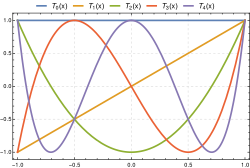
\includegraphics[width=0.6\linewidth]{static/Chebyshev-Polynomials.png}\\
    Chebyshev Polynomials $T_n(x)$ for degrees $n=1$ through $n=5$ on $[-1, 1]$.
\end{center}


You can see in the above figure \TODO{label the figures} that the extrema of the Chebyshev polynomials lie in $\{-1, 1\}$. It should be intuitive how this corresponds to the absolute value of the polynomial all sharing a common maxima.

% Optimal polynomial $p^*$ is degree 2 Chebyshev poly with $\cb{\alpha^{-1}, \beta^{-1}} = \cb{\frac{M+m}{2} \pm \frac{M-m}{2\sqrt{2}}}$.

% We can repeat all of the above arguments and find that we will get the picking $n$ steps will in general be better than $<n$ steps and the optimal polynomial will in general be a degree $n$ polynomial. Before talking more specifically about Chebyshev polynomials we talk about $p_n^*$ a little more.

% Chebyshev polynomials are defined on $[-1, 1]$ but we are interested in the range of $[m, M]$. Let's assume $L(\lambda)$ is a rescale that takes us to $[-1, 1]$ then we can talk in the language of the Chebyshev polynomials themselves. $T_n$ is the degree $n$ Chebyshev polynomial.
\TODO{add a one line exposition of Chebyshev Polynomials and $L$}

Take for granted that the solution to the minimax is 
\begin{equation}\label{eq:chebyshev-opt}
    p^*_n = \frac{T_n(L(\lambda))}{T_n(L(0))}
\end{equation}
where $L$ affinely maps the eigenvalue range $[m, M] \to [-1, 1]$ which is the natural domain of the Chebyshev polynomial.\footnote{This works out to be $L(\lambda) = \frac{\lambda - m}{M-m} \cdot 2 - 1$. For $\lambda=0$ we get $L(0) = \frac{-2m}{M-m}-1 = \frac{- M -m}{M-m} = \frac{m+M}{m-M} = \frac{1+\kappa}{1-\kappa}$}

The maximum value that $T_n$ takes on is $1$ so maximizing over $\lambda$ we get \[R^*_n = \frac{1}{T_n(L(0))}\]


We can understand the limiting optimal rate by taking the large $n$ limit:


We get that
\begin{align*}
    \lim_{n\rightarrow \infty} R^*_n &= \lim_{n\rightarrow \infty} \frac{1}{T_n(L(0))} \\
    &= \lim_{n\rightarrow \infty} \frac{2}{\p{\frac{\sqrt \kappa - 1}{\sqrt \kappa + 1}}^n + \p{\frac{\sqrt \kappa - 1}{\sqrt \kappa + 1}}^{-n} } \\
    &= 2 \left(\frac{\sqrt{\kappa}-1}{\sqrt{\kappa} + 1}\right)^n \\
    &= 2\p{1 - \frac{2}{\sqrt{\kappa}+1}}^n
\end{align*}

The second line follows from the first definition of the Chebyshev polynomials which shows up in the following section. For now it suffices to take this as true.

Taking the geometric mean over $n$ steps and dropping constants we see that the final optimal rate is  
\[\calO\p{\frac{1}{\sqrt \kappa}}\]

which is the famous ``accelerated'' rate for gradient descent.


Similarly we can get an interation complexity $R_n \leq \eps$ is $n= \Theta\p{\sqrt{k} \log(1/\eps)}$ 

\TODO{write out the justification for this using big n limit for the ``k" term.}



\textbf{Philosophical Aside:}

Why was the optimal steps for $n=2$ suboptimal for $n=1$. 

It means that we have fewer choices to pick from we have to pick something "in-between" to trade off different edge cases ("hedging").

Young 1953. 
Acceleration Methods FnTML.



\subsection{The Chebyshev Polynomials and Accelerated Methods}

Some more resources (Mason \& Handscomb, Riulin, Trefethen)


\textbf{Various Definitions of Chebyshev Polys:}
\begin{itemize}
\item \textbf{Explicit:} \[T_n(z) = \frac{\p{z-\sqrt{z^2-1}}^n + \p{z+\sqrt{z^2-1}}^n}{2}  \]
\item \textbf{Trigonometric:} \[T_n(z) = \cos(n \cdot \arccos(z)), \quad z\in[-1, 1]\]
\item \textbf{Roots:} \[\cb{\cos\p{\frac{2t+1}{2n}\pi}}_{t=0 \dots n-1}\]
	\begin{itemize}
	\item $\cb{\frac{2t+1}{2n}\pi}_{t=0\dots n-1}$ are angles spread uniformly around the unit circle. So applying $\cos$ can be thought of as projecting the points from the unit circle onto the x-axis. 
	\item Figure \ref{fig:chebyshev-roots-arcsine} is a nice picture for the distribution of roots (uniformly) on a circle then projected on to the x-axis. it is called the arcsine distribution and will come up in random step-size schedules
	\end{itemize}
\item \textbf{3-term recurrence} \[T_{n+1}(z)=2zT_n(z) - T_{n-1}(z), \quad T_0(z)=1, T_1(z) = z\]
\item \textbf{Extremal:} \[T_n(z)/2^{n-1} = \argmin_{p \text{ def } n, p \text{ monic}} \max_{z \in [-1, 1]} \abs{p(z)}\]
	\begin{itemize}
	\item This is why they showed up in our step-size derivation above.
	\end{itemize}
\end{itemize}

\begin{figure}[t]
    \centering
    \includegraphics[width=200pt]{static/Pasted image 20251027222540.png}
    \caption{Distribution of roots of Chebyshev polynomials projected onto the x-axis (arcsine distribution \TODO{fix formatting}).}
    \label{fig:chebyshev-roots-arcsine}
\end{figure}

A core message to takeaway here is that there are many equivalent ways to derive step-size schedules yielding accelerated descent \textit{and} they all correspond to some way to define the Chebyshev polynomials. This duality follow directly from the relationship between inverse roots and step-sizes. 

\subsubsection{Polyak's Heavy Ball}

To begin we can look at the Polyak Heavy Ball Method which introduced the notion of momentum to first-order optimization. Polyak's Heavy Ball can be dervied via the 3-term recurrence. 

Recall that the 3-term recurrence was 
\[T_{n+1}(z)=2zT_n(z) - T_{n-1}(z)\]

We need to shift / rescale in order to apply this recurrence to $p_{n+1}(\bH)$, our optimal contraction polynomials. We defined $L(\lambda) = a \lambda + b$ to handle scaling the input \footnote{for some values $a, b$ (we will only be concerned with the functional form for now)}. The RHS of the recurrence can then be expressed in terms of lambda $2(a\lambda + b)T_n(L(\lambda)) - T_{n-1}(L(\lambda))$, but we also need to rescale the out put as in (\ref{eq:chebyshev-opt}) so taking this into accourn the optimal polynomial recurrence is 
\[p_{n+1}(\lambda) = \p{\p{c_1+c_2\lambda}p_{n}(\lambda) - c_3 p_{n-1}(\lambda)}\]
for some values of $c_1, c_2, c_3$


Next, we want to go from this recurrence into something that we can implement. Let's start with some wishful thinking: for $n+1$ steps assume we contract according to $p_{n+1}(\bH)$ which is optimal, then write the contraction via the recurrence.
\begin{align*}
\bx_{n+1} - \bx^* &= p_{n+1}(\bH)(\bx_0-\bx^*) \\
&= \p{\p{c_1+c_2\bH}p_{n}(\bH) - c_3 p_{n-1}(\bH)}(\bx_0-\bx^*) \\
&= \p{c_1+c_2\bH}\underbrace{p_{n}(\bH)(\bx_0-\bx^*)}_{=\, \p{\bx_n - \bx^*}} - c_3\underbrace{p_{n-1}(\bH)(\bx_0-\bx^*)}_{=\, \p{\bx_{n-1} - \bx^*}}
\end{align*}

Where the third line points out that the recurrence allows us to express the optimal $n+1$ step iterate in terms of our $n$ and $n-1$ step iterates. Further rearranging gives.
\begin{align*}
    \bx_{n+1} - \bx^* &=  c_1\p{\bx_n - \bx^*} +c_2 \underbrace{\bH \p{\bx_n - \bx^*}}_{=\,\nabla f(\bx_n)} - c_3\p{\bx_{n-1} - \bx^*}\\
    &= c_1\bx_n + c'_3\bx_{n-1} + c_2 \nabla f(\bx_n) - \p{c'_3 + c_1}\bx^* \\
\end{align*}
The first line identifies the second term as the gradient for the quadratic function. In rearranging we substitute $c'_3=-c_3$ for clarity. If we constraint $c_1 + c'_3 = 1$ we can add $\bx^*$ to both sides to get
\begin{align*}
    \bx_{n+1} &=  c_1\bx_n + c'_3\bx_{n-1} + c_2 \nabla f(\bx_n)\\
    &= \bx_n  - c'_3\underbrace{\p{\bx_n- \bx_{n-1}}}_{\text{momentum}} + c_2 \nabla f(\bx_n)
\end{align*}

The final step rearranges the update rule in terms of a ``momentum'' term. Inductively, if we assumed that $\bx_n, \bx_{n-1}$ were the optimal iterates, then by construction it follows that $\bx_{n+1}$ is optimal up to $n+1$ step step-size schedule on vanilla gradient descent, thus as we take many updates $n\rightarrow \infty$ the algorithm achieves the accelerated rate.

If we were to have carried valyes for the constants throughout, we would have arrived at
\[
c'_3 = \p{\frac{2}{\sqrt{M}+\sqrt{m}}}^2, \quad c_2 =  \p{\frac{\sqrt{M}-\sqrt{m}}{\sqrt{M}+\sqrt{m}}}^2
\]



The relationship between momentum and step-size parameters $c'_3$ and $c_2$ is worth its own section. Fabian Pedregosa's 2023 ICML Blog \href{https://iclr-blogposts.github.io/2023/blog/2023/hitchhikers-momentum/}{\textit{A Hitchhiker's Guide to Momentum}} may be of interest for further reading and includes derivation of the regions for which $(c'_3, c_2)$ achieve the accelerated rate. \TODO{the derivation makes not assumption on the implementation of step-size algorithm to arrive at an optimal $n$, $n-1$ step contraction, so does it not matter?}



\TODO{Discussion of Conjugate gradients that I kind of missed, but conjugate gradients are based on orthogonal polynomials}

\subsubsection{Random Stepsizes via Potential Theory}

Note that the derivation for optimal step-size schedules in \ref{subsubsec: The General Case} \textbf{never} made an assmption on the ordering of step-sizes. Informally,
as number $n$ steps we are optimizing grows large, taking a random ordering of these step-sizes can be approximated by sampling iid from some distribution - that is something like  $\mu_n = \frac{1}{n}\sum_t\delta(\alpha_t)$ for large $n$. The figure \ref{fig:chebyshev-roots-arcsine} would suggest that the limiting distribution $\mu_n \rightarrow \mu$ is the arcsine distribution.

Alternatively, we can give theoretical justification for $\mu$ by showing that it is the optimal distribution. To begin, will express our problem using the matrix norm.

\begin{align*}
    R_n(\omega) &= \max_{f} \norm{\prod{\p{\bI-\alpha_t(\omega) \bLambda}}} \\
    &= \max_{\lambda\in[m,M]} \norm{\prod{\abs{1- \alpha_t(\omega)\lambda}}}
\end{align*}

Where $\alpha_t(\omega)$ are function of the random draw from $\mu$, and the second line diagonalizes.
The optimization problem we will be interested in for the random case is 
\[\min_\mu \lim_{n\to\infty} \E_{\{\alpha_t\}\sim\mu^n} \b{\sqrt[n]{R_n}}\]
% \footnote{It is tempting to only consider the expected contraction only one-step but the result may be misleading. Consider the betting game where everyday you may 2x your wealth or 1/4x it. For a large number of days, do you earn money?}


% \[R(\mu) = \max_{f, \bx_0} \lim_{n\rightarrow \infty} \E_{\{\alpha_t\} \sim \mu^n}\b{\frac{\norm{\bx_n - \bx^*}}{\norm{\bx_0-\bx^*}}^{1/n}}\]

% What is the optimal $\mu$ to sample from? What is the corresponding rate? 

% We should first move this to the matrix norm formulation and diagonalize, which in this case results in an upper bound.
% \footnote{There is additional nuance to moving to a matrix norm since it technically requires moving the $\max_{x_0}$ from outside the limit and expectation to inside to arrive at something like $\max_{f} \lim_{n\rightarrow \infty} \E_{\{\alpha_t\} \sim \mu^n}\b{\p{\max_{x_0}\frac{\norm{\bx_n - \bx^*}}{\norm{\bx_0-\bx^*}}}^{1/n}}$. To move the $\max_{x_0}$ inside the limit we can upper bound the $\lim_{n\rightarrow\infty}$ by replacing it with a  $\lim \sup_{n\rightarrow\infty}$ since $\max$ can commute with $\lim \sup$. To move the max inside the expectation we can leverage the fact that $\max_{x_0} \E_\alpha[f(x_0, \alpha)] \leq \E_\alpha[\max_{x_0} f(x_0, \alpha)].$ for any $f$.}

% \[R(\mu) \leq \max_{f} \lim_{n\rightarrow \infty} \E\b{\norm{\prod{\p{\bI-\alpha_t \bLambda}}}^{1/n}}\]






% This reduces down to a scalar optimization over the worst case eigenvalue. In the scalar setting we can move the absolute values inside of the product

% \[R(\mu) = \max_{\lambda \in [m, M]} \lim_{n\rightarrow \infty} \E\b{\p{\prod{\abs{1- \frac{\lambda}{\beta_t}}}}^{1/n}}\]


We want to study how the geometric mean converges. To do this, we can analyze the log one-step contraction rate. In general, if $X_i$ are distributed i.i.d and $G_n := \p{\prod X_i}^{1/n}$ is the geometric mean, then $\E \log X_i = m$ implies that $G_n \to e^m$ almost surely.\footnote{See further discussion at \href{https://math.stackexchange.com/questions/1108732/geometric-mean-with-the-law-of-large-numbers}{this Math Stack Exchange post}.} Thus it suffices to study the problem minimizing 

\[\log R(u) = \max_{\lambda\in[m, M]} \E \p{\log\abs{1-\frac{\lambda}{\alpha}}}\]

since it will also minimize the geometric average of the rates. To solve the problem cleanly we can make a connection to electrostatic potential theory. To begin, we write the two problems as follow:

\begin{itemize}
\item Step-size Problem: copy paste from aboves but we use $\beta = \alpha^{-1}$ to minimize over the inverse-step-size distribution $\gamma$ since it allows us to make a cleaner connection to potentual theory.
\[\min_{\gamma} \max_{\lambda \in [m, M]}  \E_{\beta\sim\gamma} \log \abs{1-\frac{\lambda}{\beta}}\]


\item Electrostatics Problem: Meinimization of potentials on a line where the $\log1/\abs{\beta-\alpha}$ kernel defines the energy between particles \[\min_{\gamma \in \calP(m, M)} \E_{\alpha, \beta \sim \gamma} \log\frac{1}{\abs{\beta-\alpha}} \]

\end{itemize}

\textbf{Fundamental Theorem of Potential Theory:} Characterized uniquely by an equalizing property \[\lambda \mapsto \E \log \p{\frac{1}{\abs{\beta-\alpha}}}\]

In other words, suppose we sample from the continuum of points leading to the same log potential no matter where you are on the graph. One way to think about this intuitively is that this is a ``stationary'' potential since (if we allow particles to move around) there is no place where the potential is higher / lower than where it is in the distribution.

Jason provided some intuitive argument for the actual conclusion that arcsine is the optimal $\gamma$ but it was more complex \TODO{look deeper into this here is a link from a 
\href{https://chatgpt.com/s/t_690bce76645c81919b6cb31f3676705e}{Chat} 
}

\textbf{Connection to perfect hedging:}

\includegraphics[width=400pt]{static/Screenshot 2025-10-30 at 4.43.11 PM.png}

In the limit of Chebyshev step sizes what ends up happening is that we are ``equally" hedged against everything. This means that \textbf{CHEBYSHEV BASED METHODS NEVER DO BETTER} than \[\frac{\sqrt{k} -1}{\sqrt{k} + 1}\]

There is some connection to Green's function that I should learn about: fundamentally, the step size optimum is given by the negative green's function evaluated on $[m, M]^c$ or something like this on the complex plane. \TODO{learn more about this}


\subsection{Understanding the best case scenarios via a two player game}
\begin{itemize}
\item Min plays a step-size distribution
\item Max plays a quadratic function
\end{itemize}

Game \[ Rate = \inf_{\gamma} \sup_{\lambda \in [m, M]} \E_{\beta \sim\gamma} \log\abs{1-\beta^{-1}\lambda}\]
To make the game more symmetric we can lift the function player into distribution over $\lambda$s giving \[\inf_{\gamma\in \calP(E)} \sup_{\rho \in \calP(E)} \E_{\beta\sim\gamma, \lambda\sim\rho} \log\abs{1-\beta^{-1}\lambda}\]

% \section{Performance Estimation Problem (PEP)}

% Can we automatically figure out worse-case functions 

% \textbf{Performance Estimation Problem for Gradient Descent:}


% Consider the worst-case function $f$ which is $L$-smooth and $\mu$-strongly convex. Given initialization $x_0$, first iterate $x_1$, and the minimizer $x^*$, the max performance estimation problem for the normalized residual after one step of gradient descent is:


% The primal for these problems is the worse case function a algorithm performs.
% The dual is the best worst-case bound you can get from an algorithm.

% \TODO{Fix this cursor generated}
% \begin{align*}
%     R_1(\mu) = \max_{f,\, x_0,\, x_1,\, x^*} \quad & \frac{\norm{x_1 - x^*}^2}{\norm{x_0 - x^*}^2} \\
%     \text{subject to} \quad & f \text{ is } L\text{-smooth}, \\
%     & f \text{ is } \mu\text{-strongly convex}, \\
%     & x_1 = x_0 - \alpha \nabla f(x_0), \\
%     & x^* = \arg\min_x f(x).
% \end{align*}


% $f$ is a hard function class to optimize over so we can re-write this as.


% The notes for this are primarily covered in some prof. Adrian's notes \href{https://adrientaylor.github.io/share/general_slides.pdf}{here}.

% Jason provided some additional insight on Sum of Square's programming as a way to get a ``certificate'' for a bound between polynomials.


% \section{Silver Step-sizes}

% Question: can you accelerate GD without changing algorithm. Just changing step sizes.

% Consider in $m$-smooth, $M$-strongly convex setting. Same GD step as original. $\kappa = M/m$.

% Mainstream from convex opt:
% \[\alpha_t = \overline{\alpha} \]
% which leads to $\Theta (\kappa)$ iterations to converge. This is the slow ``unaccelerated'' rate.
% We want to get the accelerated rate on general Convex problems.

% Before $\Theta (\sqrt k)$ has shown using methods with additional dynamics on general convex functions via Nesterov's accleration.

% If we look back at our analysis polynomials, it breaks down in convex functions because our Hessians $H$ change from step to step.

% Only the one-step case holds which is why we know the rate is at most $\theta(\kappa)$ in vanilla GD.

% One important idea is that if we consider the one-step optimal rate computed by finding the smallest $R_1$ to bound 
% \[\norm{x_1 - x^*} \leq R_1 \norm{x_0-x^*}\]

% This is suboptimal. In particular $R_1$ is optimized to be greedy for one-step as opposed to over schedules. In this sense, $R_1$ is the greedy contraction rate.

% Although there were empirical solutions to get step-sizes for faster performance in practice, there was NO step-size algorithm to get anything faster than.

% That is until Jason's paper in 2018.

% First we make some observations about how convex functions compare to quadratics with regard to a two step optimal solution. Jason hides the math here.

% Jason goes on to define silver step-sizes.


% There is a recusrive fomulaiton for n*2 steps where you take the n step schedule repeat twice and then within each of the two sub-n-step-schedules you multiply the last 


% Some information about the actual analysis

% Formulate the min-max problem just as before. 

% $\min_\{\alpha\} \max_{f, x_0} rate(\mu)$


% There is a lot of interesting research in this area.


% \section{Optimization on Manifolds}

% \section{Negative Stepsizes}

% \section{Ravines in Optimization}

\section{Nesterov's Accelertion and Curvature}

This section is based on work from \href{https://arxiv.org/pdf/1503.01243}{Su, Boyd and Candes} (2015) and \href{https://arxiv.org/pdf/1810.08907}{Shi et al.} (2018).


Acceleration over the class of $L$-smooth convex functions has proven to be a more challenging 
problem. In 1983, Yurii Nesterov proposed a simple modification to the gradient descent rule yielding the $O(1\sqrt{T})$ rate to match the quadratic setting. Termed, Nesterov acceleration, the update can be written as:
\begin{align*}
    \by_k   &= \bx_k + \beta_k (\bx_k - \bx_{k-1}) \\
    \bx_{k+1} &= \by_k - \eta \nabla f(\by_k)
\end{align*}

where $\beta_k$ is a momentum parameter (which can be tuned or scheduled) and $L$ is the smoothness parameter of $f$.

Visually, this update first extrapolates $\bx_k$ in the direction of its last iteration ($\bx_k - \bx_{k-1}$) to get $\by_k$, and then performs a gradient step from the extrapolated point $\by_k$. We can visualize the updates on quadratic $f(\bx) = 10x_1^2 + x_2^2$ in Figure \ref{fig:nest_step_example_and_comparison}

The proof for NAG is complicated, so we are going to leave it out for now, but there is useful intuition in comparing the algorithm to Polyak's heavy ball. The updates are almost identical except in Nesterov's the gradient is computed at the point $\textcolor{red}{\by_k}$ as opposed to $\textcolor{blue}{\bx_k}$.
\begin{align*}
   \text{Polyak's Update} &\quad \bx_{k+1} = \by_k - \eta \nabla f(\textcolor{blue}{\bx_k}) \\
   \text{Nesterov's Update} &\quad \bx_{k+1} = \by_k - \eta \nabla f(\textcolor{red}{\by_k})
\end{align*}

\begin{figure}[t]
    \centering
    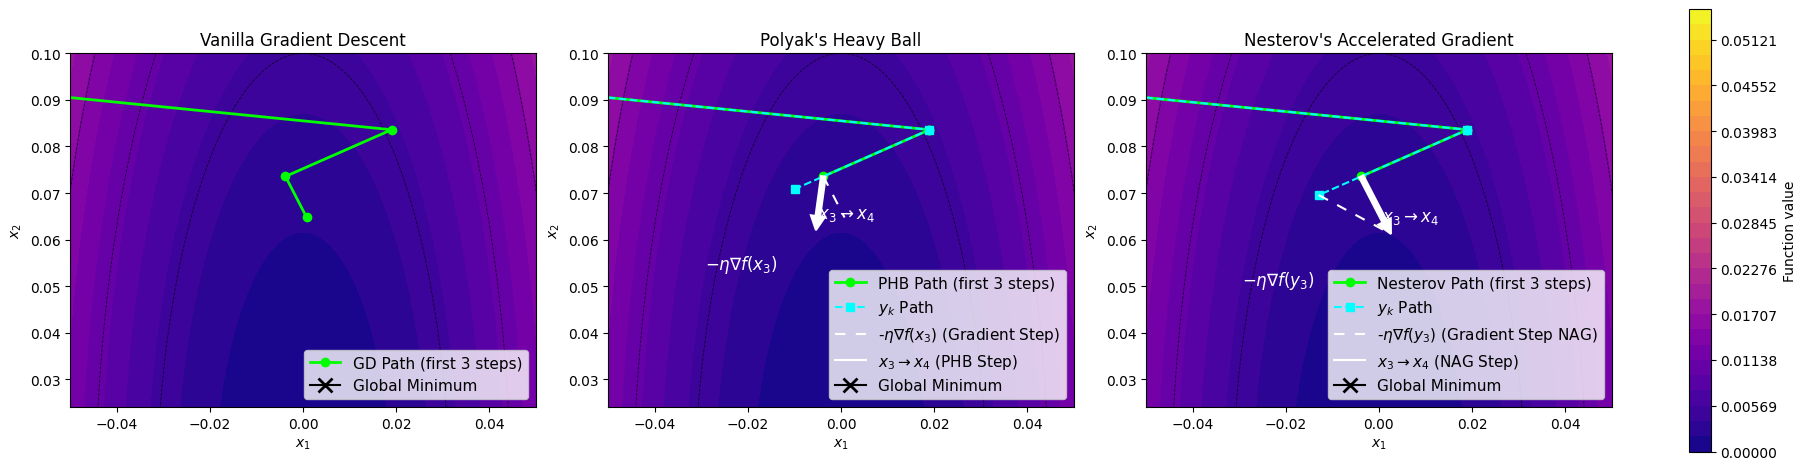
\includegraphics[width=0.7\textwidth]{static/nest_step_example.png}
    \\[1.2em]
    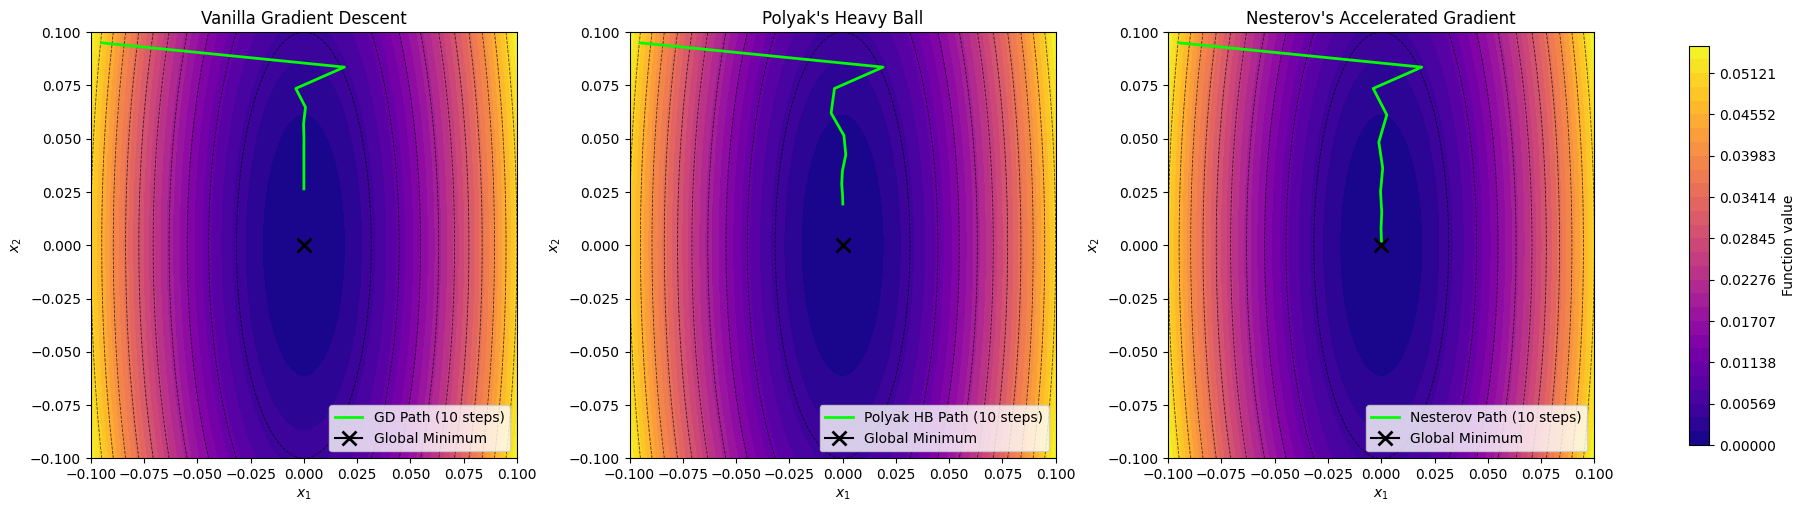
\includegraphics[width=0.7\textwidth]{static/vgd_nest_phb_comparison.png}
    \caption{
        Top row: Illustration of Nesterov's accelerated gradient descent steps on the quadratic function $f(\bx) = 10x_1^2 + x_2^2$. Bottom row: Comparison between 10 steps of vanilla gradient descent, Nesterov acceleration, and Polyak heavy ball methods on the same function
        }
    \label{fig:nest_step_example_and_comparison}
    \end{figure}

As in previous algorithms the challenge of adapting quadratic methods to general convex functions is that curvature may vary from one point to another. Intuitively, we might hope that $\nabla f(\by_k)$ provides more of curvature information than $\nabla f(\bx_k)$.

We can start to see this by writing $\nabla f(\by_k)$ as a taylor approximation around $\nabla f(\by_k)$.
\begin{align*}
    \nabla f(\by_k) &\approx \nabla f(\bx_k) + \nabla^2 f(\bx_k)(\by_k - \bx_k) \\
    &= \nabla f(\bx_k) + \nabla^2 f(\bx_k)\, \beta_k (\bx_k - \bx_{k-1})
\end{align*}

For the quadratic case, this approximation is exact.

\TODO{Add a plot here to indicate whether this actually works or not as an algorithm on general convex functions since it should trivially work on quadratics}



\end{document}